\documentclass[a4paper,11pt,fleqn]{article}%fleqn pour aligner les equations à gauche
\usepackage{../../Styles/Cours}

\newcommand{\chnum}{Chapitre 2}
\newcommand{\chtitle}{Quel usage pour une solution antiseptique ?}
\newcommand{\dtype}{TP}


\begin{document}
\maketitle
Le permanganate de potassium (\ce{KMnO4}), ou cristal de Condy, est un antiseptique utilisé dans des produits pour désinfecter des plaies, les fruits et légumes, traider des eaux, etc. Les propriétés des désinfectants dépendent de leur concentration.\\
La teneur en permanganate de potassium d'un sachet du commerce est vérifiable par analyse chimique.\\
Une solution a été préparée dans un flacon non étiquetée. Comment vérifiée, à l'aide de stratégies d'analyses physiques différentes, pour quel usage elle a été préparée ?

\begin{figure}[h!]
    \begin{minipage}{.48\linewidth}
    \begin{minipage}{\linewidth}
        \caption{Un sachet de cristal de Condy}
        \textbf{Conditionnement :}\\
        Sachet de \SI{0,25}{\gram} de \ce{KMnO4} en poudre\\
        Masse molaire : $M(\ce{KMnO4})= \SI{158,0}{\gram\per\mole}$\\

        \textbf{Utilisations :}\\
        Dissoudre dans l'eau le contenu du sachet dans : 
        \begin{itemize}
            \item \SI{0,6}{L} pour désinfécter des fruits et légumes
            \item \SI{1,0}{L} pour un usage antiseptique cutané
            \item \SI{2,0}{L} pour éliminer les algues, bactéries et champignons sur les parois d'un aquarium, ajouter ensuite \SI{20}{mL} de la solution préparée par litre d'eau de l'aquarium
        \end{itemize}
    \end{minipage}

\vspace{2em}
    \begin{minipage}{\linewidth}
        \caption{Spectre d'absorption d'une solution aqueuse de permanganate de potassium}
        \begin{center}
            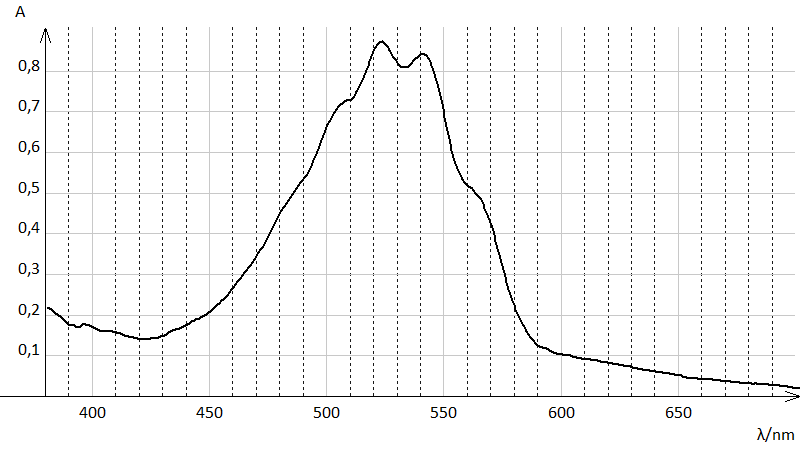
\includegraphics[width=\linewidth]{Ressources/TSPE_C2_S&C_Fig1.png}
        \end{center}
    \end{minipage}
    \end{minipage}\hspace{2em}
    \begin{minipage}{.48\linewidth}
        \caption{Matériel}
        Solution mère $S_0$ de permanganate de potassium de concentration \SI{1,5}{\milli\mole\per\liter}. 4 solutions étalons de concentration en quantité de matière :
        \begin{itemize}
            \item $S_1$ : \SI{0,300}{\milli\mole\per\liter}
            \item $S_2$ : \SI{0,225}{\milli\mole\per\liter}
            \item $S_3$ : \SI{0,150}{\milli\mole\per\liter}
            \item $S_4$ : \SI{0,0750}{\milli\mole\per\liter}
        \end{itemize}
        \vspace{2em}
        \begin{itemize}
            \item Fiole jaugée de \SI{100,0}{mL} munie d'un bouchon
            \item Bécher de \SI{150}{mL}
            \item Pipette jaugée de \SI{10,0}{mL}
            \item Papier absorbant
            \item Solution étalon de conductimétrie
            \item Sonde de conductimétrie
            \item Spectrophotomètre et cuves
        \end{itemize}
    \end{minipage}
    
\end{figure}

\begin{enumerate}
    \item Identifier deux méthodes physiques envisageables pour déterminer la concentration en quantité d'ion permanganate et d'ion potassium dans la solution inconnue en justifiant les choix.
    \item Justifier que la solution à étudier est trop concentrée.
    \item Cette solution sera donc diluée dix fois avant analyse. Proposer un protocole détaillant la verrerie nécessaire pour réaliser cette dilution.
    \item Mettre en \oe uvre le protocole après valisation par le professeur.
    \item Déterminer la concentration en masse en permanganate de potassium dans le flacon non étiqueté puis l'usage prévu pour e flacon.
    \item Comparer les méthodes utilisées.
\end{enumerate}

\begin{center}
    \renewcommand{\arraystretch}{3}
    \begin{tabular}{|>{\centering}m{.15\linewidth}|>{\centering}m{.08\linewidth}|>{\centering}m{.08\linewidth}|>{\centering}m{.08\linewidth}|>{\centering}m{.08\linewidth}|>{\centering}m{.08\linewidth}|>{\centering}m{.08\linewidth}|>{\centering\arraybackslash}m{.08\linewidth}|}
    \hline
    \textbf{Solution} & \textbf{Eau} & $\mathbf{S_0}$ & $\mathbf{S_1}$& $\mathbf{S_2}$& $\mathbf{S_3}$& $\mathbf{S_4}$& $\mathbf{X}$\\
    \hline
    \textbf{Concentration} (\unit{\milli\mole\per\liter}) & 0 & 1,5 & 0,300 & 0,225 & 0,150 & 0,075 & \\
    \hline\textbf{A} & & & & & & & \\
    \hline
    $\mathbf{\sigma}$ (\unit{\milli\siemens\per\centi\meter})  & & & & & & & \\
    \hline
\end{tabular}
\end{center}

\end{document}